\documentclass{szzclass}
\usepackage{hyperref}
\usepackage{longtable}
\usepackage{booktabs}

\subject{MLO}
\code{BI-SPOL-15}
\topic{Predikátová logika: jazyk, interpretace, pravdivost formulí, logický důsledek a ekvivalence. Formalizace matematických tvrzení a jejich negace. Teorie a jejich modely (např. uspořádání).}

\providecommand{\tightlist}{%
  \setlength{\itemsep}{0pt}\setlength{\parskip}{0pt}}

\begin{document}
\tableofcontents
\newpage

\section{Jazyk predikátové logiky}
Jazyk obsahuje \textit{logické symboly} a \textit{mimologické symboly L}.
\begin{itemize}
  \item symboly pro \textit{proměnné} (x, y, z)
  \item symboly pro \textit{logické spojky} ($\neg, \wedge, \vee, \Rightarrow, \Leftarrow$)
  \item symboly pro \textit{kvantifikátory} vždy následuje proměnná
  \begin{itemize}
    \item obecný - "všichni" $\forall$
    \item existenční - "některé/existuje" $\exists$
  \end{itemize}
  \item pomocné symboly - závorky
  \item symboly pro \textit{konstanty} (K, S, \dots)
  \item symboly pro \textit{predikáty} ($p, q, r$) - dána četnost
  \item symboly pro \textit{funkce} ($f, g, \dots$)
\end{itemize}
\subsection{Term}
Řetězec symbolů se nazývá \texttt{term} jestliže vznikne použitím těchto pravidel v konečně mnoho krocích:
\begin{itemize}
  \item každá proměnná a konstanta je term
  \item jsou-li $t_1, t_2,\dots,t_n$ termy a $f$ je $n$-ární funkční symbol, potom $f(t_1,\dots,t_n)$ je term
\end{itemize}
\subsection{Formule}
\texttt{Formule} je posloupnost symbolů, která vznikne aplikací následujících pravidel v konečné mnoha krocích:
\begin{itemize}
  \item je-li $n$-ární predikátový symbol a $t_1,...,t_n$ jsou termy, pak $p(t_1,...,t_n)$ je formule - atomická formule
  \item jsou-li A a B formule, pak $\neg A, (A \wedge B), (A \vee B)\dots$ jsou formule
  \item je-li $x$ proměnná a A formule, pak $(\forall{x})$A a $(\exists{x})$A jsou formule
\end{itemize}
\subsection{Volné a vázané proměnné}
\begin{itemize}
  \item podformule B je část formule A, která je sama formulí
  \item proměnná x má vázaný výskyt v A právě, když se vyskytuje v její podformuli ve tvaru $(\forall{x})B(x)$ nebo $(\exists{x})B(x)$
  \item výskyt proměnné v A, který není vázaný, je volný výskyt
\end{itemize}
\begin{itemize}
  \item uzavřená formule obsahuje pouze vázané proměnné
  \item otevřená formule obsahuje pouze volné proměnné
\end{itemize}
\section{Interpretace jazyka}
Interpretace (realizace, struktura) M = $<M,\dots,K_M,\dots,p_M,\dots,f_M,\dots>$ jazyka L obsahuje:
\begin{itemize}
  \item neprázdnou množinu M, kterou nazýváme universum interpretace,
  \item je-li K konstanta, pak její interpretaci $K_M \in M$
  \item je-li p $n$-ární predikát, pak $n$-ární relaci $p_M \subseteq M^n \rightarrow M$ jako jeho interpretaci
  \item je-li f funkce mající n argumentů, pak funkci $f_M: M^n \rightarrow M$ jako její interpretaci
\end{itemize}
Jeden jazyk může mít více interpretací
\section{Pravdivost formulí}
L je jazyk a M je jeho interpretace
\begin{itemize}
  \item ohodnocení proměnných je funkce $e$ z množiny proměnných, které každé volné proměnné přiřazuje nějaký prvek univerza M
  \item výrazem $t[e]$ označujeme hodnotu termu $t$ při ohodnocení $e$.
  \begin{itemize}
    \item je-li term $t$ proměnná $x$, pak $t[e]$ = $e(x)$
    \item je-li n-ární funkční symbol a term $t$ je $f(t_1,...,t_n)$, pak $t[e] = f(t_1[e],...,t_n[e])$
  \end{itemize}
  \item výraz e(x/m) se označuje hodnocení, které všem proměnným přiřadí stejnou hodnotu jako e, jenom e(x) = m
\end{itemize}
Pravdivost formule v interpretaci M při ohodnocení e se definuje indukcí podle složitosti formule
\begin{figure}[!h]
  \centering
  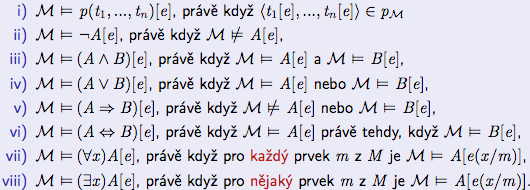
\includegraphics[width=\textwidth]{topics/bi-spol-15/images/logicalEvaluation.png}
  \caption{Tarského definice pravdy}
\end{figure}
Formule A je pravdivá (platná) v interpretaci M, právě když pro každé ohodnocení e je pravdivá, tj. $M \models A[e]$.
\newline
Formule A je splnitelná, právě když v nějaké interpretaci M pro nějaké ohodnocení e je pravdivá.
\newline
A je kontradikce, právě když není splnitelná.
\section{Logická ekvivalence, logický důsledek}
\begin{itemize}
  \item A a B jsou logicky ekvivaletní, $A \models B \wedge B \models A$, právě když pro každou interpretaci M a pro každé ohodnocení e platí: $M \models A[e]$, právě když $M \models B[e]$
  \item B je logickým důsledkem A, $A \models B$, právě když pro každou interpretaci M a pro každé ohodnocení e platí: jestliže $M \models A[e]$, pak $M \models B[e]$
\end{itemize}
\section{Příklad matematického příkladu}
\begin{itemize}
  \item $(\exists{u})(x = u + u)$ - x je sudé = negace = $(\forall{u})\neg(x = u + u)$
  \item $\neg(\exists{u})(x = u + u)$ - x je liché
  \item $(\exists{x})(x = y*z)$ - x dělí y
\end{itemize}
\section{Teorie a Model}
\begin{itemize}
  \item teorie je množina uzavřených formulí
  \item interpretace M jazyka L je modelem T, jestliže každá formule platí v M
  \item formule A je logický důsledek teroie T, jestliže v každém modelu teorie T platí A
  \item teorie T je splnitelná, právě když má model
\end{itemize}
Teorie ekvivalence:
\begin{itemize}
  \item L = {r(x,y)}. Predikát r(x, y) je ekvivalence, jestliže platí
  \begin{itemize}
    \item R: $(\forall{x}) r(x,x)$ - reflexifita
    \item T: $(\forall{x})(\forall{y})(\forall{z})(r(x,y) \wedge r(x,y) \Rightarrow r(x,z))$ - tranzitivita
    \item S $(\forall{x})(\forall{y})(r(x,y) \Rightarrow r(y,x))$ - symetrie
  \end{itemize}
\end{itemize}
Teorie neostrého uspořádání
\begin{itemize}
  \item L = {q(x, y)}. Pro teorii neostrého uspořádání platí následující axiomy
  \begin{itemize}
    \item R: $(\forall{x}) r(x,x)$ - reflexifita
    \item T: $(\forall{x})(\forall{y})(\forall{z})(r(x,y) \wedge r(y,z) \Rightarrow r(x,z))$ - tranzitivita
    \item As $(\forall{x})(\forall{y})(r(x,y) \wedge r(y,x) \Rightarrow (x = y))$ - slabá asymetrie
  \end{itemize}
\end{itemize}
Teorie ostrého uspořádání
\begin{itemize}
  \item pro teorii ostrého uspořádání platí následující axiomy
  \begin{itemize}
    \item T: $(\forall{x})(\forall{y})(\forall{z})(r(x,y) \wedge r(x,y) \Rightarrow r(x,z))$ - tranzitivita
    \item IR: $(\forall{x})\neg p(x,x)$ - ireflexivita
  \end{itemize}
\end{itemize}
Teorie neomezeného hustého lineárního uspořádání je teorie hustého lineárního uspořádání, pro kterou navíc platí:
$(\forall{x})(\exists{y})(\exists{z})(y < x \wedge x < z)$ - neomezenost.
\end{document}
